%epsilon est le taux min des pertes par effets joules pour lequel l'oracle ne comet pas d'erreurs.
% EJ ce sont les pertes par effet joules dans le reseau.

% DECISION : ABANDON DE CE PARAGRAPHE car utilise les algorithmes de couvertures
Nous consid\'erons que le r\'eseau \'electrique modelis\'e par un DAG $G$ est connu.
Nous \'etudions l'\'evolution du pourcentage minimum des pertes par effets joules not\'ee $\epsilon$ en fonction des partitions coh\'erente propos\'ee par  {\em Verif-correl}.
Nous d\'efinissons la {\em similarit\'e} comme \'etant le pourcentage d'arcs de $A$ bien pr\'edits par $Verif-correl$.
Nous r\'ealisons deux exp\'eriences: 
\begin{itemize}
\item La premi\`ere exp\'erience consiste \`a g\'en\'erer des mesures de flots de divers graphes en faisant varier, de $0$ \`a $1$ par pas de $0.125$, les pertes par effets joules $EJ$ tout en fixant la variable $\epsilon$. Nous ex\'ecutons l'algorithme de couverture sur diff\'erents graphes, chaque graphe ayant un $EJ \in [0,1]$. Nous \'etudions l'\'evolution de la  similarit\'e en fonction de pertes joules $EJ$. 

\item La deuxi\`eme exp\'erience consiste \`a faire varier la variable $\epsilon$ en fixant la similarit\'e \`a $1$.  Nous \'etudions les variations des pertes en fonctions de $\epsilon$.  Les pertes par effets joules $EJ$ varient  de $0$ \`a $1$ par pas de $0.125$. 

\end{itemize}
Rappelons que $EJ=0.1$ signifie qu'il existe une diff\'erence de flot par grandeurs de $0.1$ entre les arcs ext\'erieures (sortantes) et int\'erieures (entrantes) \`a chaque sommet. Ainsi $EJ=0$ signifiant qu'il n'existe aucune perte tandis que  $EJ=1$ signifiant qu'il n'existe aucuns flots entre les arcs entrants et sortants d'un sommet du r\'eseau de flots.
% experience 1
\paragraph{exp\'erience 1} :
On fixe  $\epsilon=0.75$. 
La figure \ref{courbeEJCoef} resume les variations de {\em Verif-correl}. 
Le fait que la courbe de la variable $\epsilon$ est d\'ecroissante confirme notre hypoth\`ese selon laquelle il n'existe aucuns flots entre les arcs entrants et sortants d'un sommet lorsque les pertes par effets joules sont \'egales \`a $EJ = 1$. En effet, pour toute valeur de pertes par effets joules  $EJ=[0,0.3]$, le graphe propos\'e est identique au graphe du r\'eseau \'electrique. Par contre, {\em Verif-correl} se trompe deux sur trois sur les cliques fournies pour $EJ = ]0.3,0.9]$ parce que la coefficent de similarit\'e est de $0.38$. 
\begin{figure}
\centering
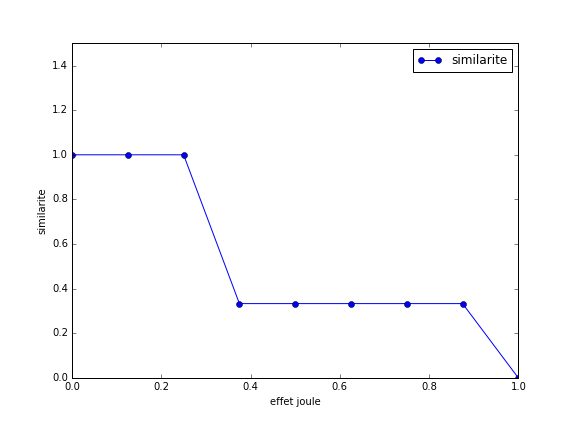
\includegraphics[scale=0.50]{courbe_similarite_selon_EJ_pour_epsilon_075.png}
\caption{ Le coefficient de similarit\'e en fonction des pertes par {\em effets joules} pour $epsilon=0.75$.}
\label {courbeEJCoef}
\end{figure}
\FloatBarrier

%experience 2
\paragraph{exp\'erience 2} :
Ici, on suppose la similarit\'e \'egale \`a $1$ et on cherche les variations de la variable $\epsilon$ en fonction des pertes par {\em effets joules}. 
Les pertes par {\em effets joules} varient de $[0,1]$ par pas de $0.125$ et nous distinguons $8$ intervalles [0,0.125], ]0.125,0.250], ]0.250,0.375], ]0.375,0.5], ]0.5,0.625], ]0.625, 0.75], ]0.75,0.875], ]0.875,1]. 
Pour chaque valeur $\epsilon$, on compte les intervalles $EJ_x, x \in [1,8]$ dans lesquelles la similarit\'e est \'egale \`a $1$ not\'e $X(\epsilon)$. Ainsi $X(\epsilon=0.3) = 8$ signifie que  les pertes par effets joules varient de $0$ \`a $1$ (EJ=[0,1]) et $X(\epsilon=0.3) = 2$ correspond \`a une variation de $EJ$ sur l'intervalle $[0,0.250]$.
On cr\'ee ainsi la distribution de $\epsilon$ en fonction des pertes par effets joules.
La figure \ref{courbeEpsilonEJ}  r\'esume cette distribution qui varie de $1$ (correspondant \`a une variation sur [0,0.125]) \`a $8$ (correspondant \`a une variation sur [0,1]).
La courbe de cette distribution est constante de l'intervalle $\epsilon = [0,0.125]$ puis  d\'ecroissante de l'intervalle $\epsilon =[0.125,1]$ et cette pente est tr\`es accentu\'ee dans l'intervalle $\epsilon = [0.8, 1]$. 
Au d\'el\`a  de $\epsilon > 0.8$, les pertes par effets joules varient dans l'intervalle $EJ=[0,0.2]$.
On en conclut que le meilleur intervalle est $\epsilon = [0.8, 1]$ pour produire des graphes de similarit\'e \'egale \`a $1$ en pr\'esence de pertes par {\em effets joules} de $20\%$.
\newline
% images
\begin{figure}
\centering
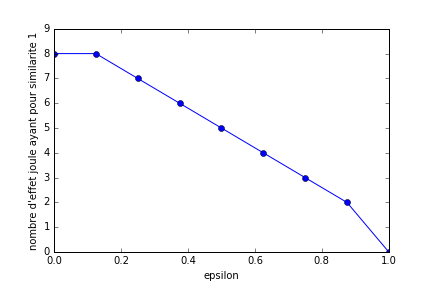
\includegraphics[scale=0.60]{courbe_epsilon_selon_nbreEJ_pour_similarite_1.png}
\caption{ Relation inverse entre $\epsilon$ et $EJ$: $8$ en ordonn\'e correspond \`a $[0,1]$, $7$ \`a $[0, 0.875]$ }
\label {courbeEpsilonEJ}
\end{figure}
\FloatBarrier

% conclusion
{\bf Conclusion} : Ces deux exp\'eriences montrent que la d\'ecision de la fonction {\em Verif-correl}  a une r\'elation inverse avec les pertes par effets joules ($EJ$). En effet, plus $\epsilon$ est petit plus les pertes par effets joules sont grandes et plus les d\'ecisions de {\em Verif-correl} sont erron\'ees.
\begin{equation}
	\epsilon > 1 - EJ
\end{equation}
